%% content.tex
%%

%% ===========================         
\chapter{Konzeption}
\label{ch:Konzeption}
%% ===========================

Ein Konzept dient in der Softwarearchitektur der Konstruktion eines abstrakten Systemmodells. Zur Gestaltung werden technische Details weggelassen und stattdessen allgemeingültige Begriffe und ihre Zusammenhänge festgelegt. Weiterhin wird ein Grundverständnis durch Definieren von Strukturen und Konzepten gebildet. Darüber hinaus werden Schnittstellen definiert, die Wechselwirkungen zwischen den Komponenten beschreiben. Weiterhin werden im Zuge der Überlegungen Technologien ausgewählt, die zur Umsetzung der verschiedenen Komponenten verwendet werden.

%% ===========================
\section{Architektur}
\label{ch:Konzeption:architektur}
%% ===========================

Zuerst wird ein erster Überblick über den geplanten Aufbau des Systems gegeben. Abbildung \ref{konzept_architektur} zeigt die Komponenten des Systems und der Umwelt. Der Tomcat mit seinen Webcontainern bildet die Basis des Systems. Wie auf der Abbildung zu sehen sind zwei verschiedene Projekte vorgesehen. Zum einen ein Client-Webprojekt und zum anderen ein Server-Webprojekt. Das Client-Webprojekt soll die Klassen und Methoden zur Umsetzung der Darstellung beinhalten. Die Anwendungslogik sowie die Datenbank sind im Server-Webprojekt vorgesehen. Der Grund für die Aufteilung in zwei verschiedene Webprojekte ist die Anforderung einer losen Kopplung zwischen Client und Server. Beide Webprojekt werden in Form von Web-Archive-Dateien in einem Apache-Tomcat-Webserver deployed und können über die entsprechende URL angesprochen werden. Weiterhin soll ein selbstgeschriebenes Plugin für den CAS genesisWorld Anwendungsserver die Aktualität des Systems garantieren. Der Browser, CAS genesisWorld und der MSSQL-Server stellen die Umwelt des Systems dar. Im Folgenden wird auf jede Komponente der Architektur eingegangen und ihre Rolle im Gebilde erläutert.

\begin{figure}[htbp]
\centering
  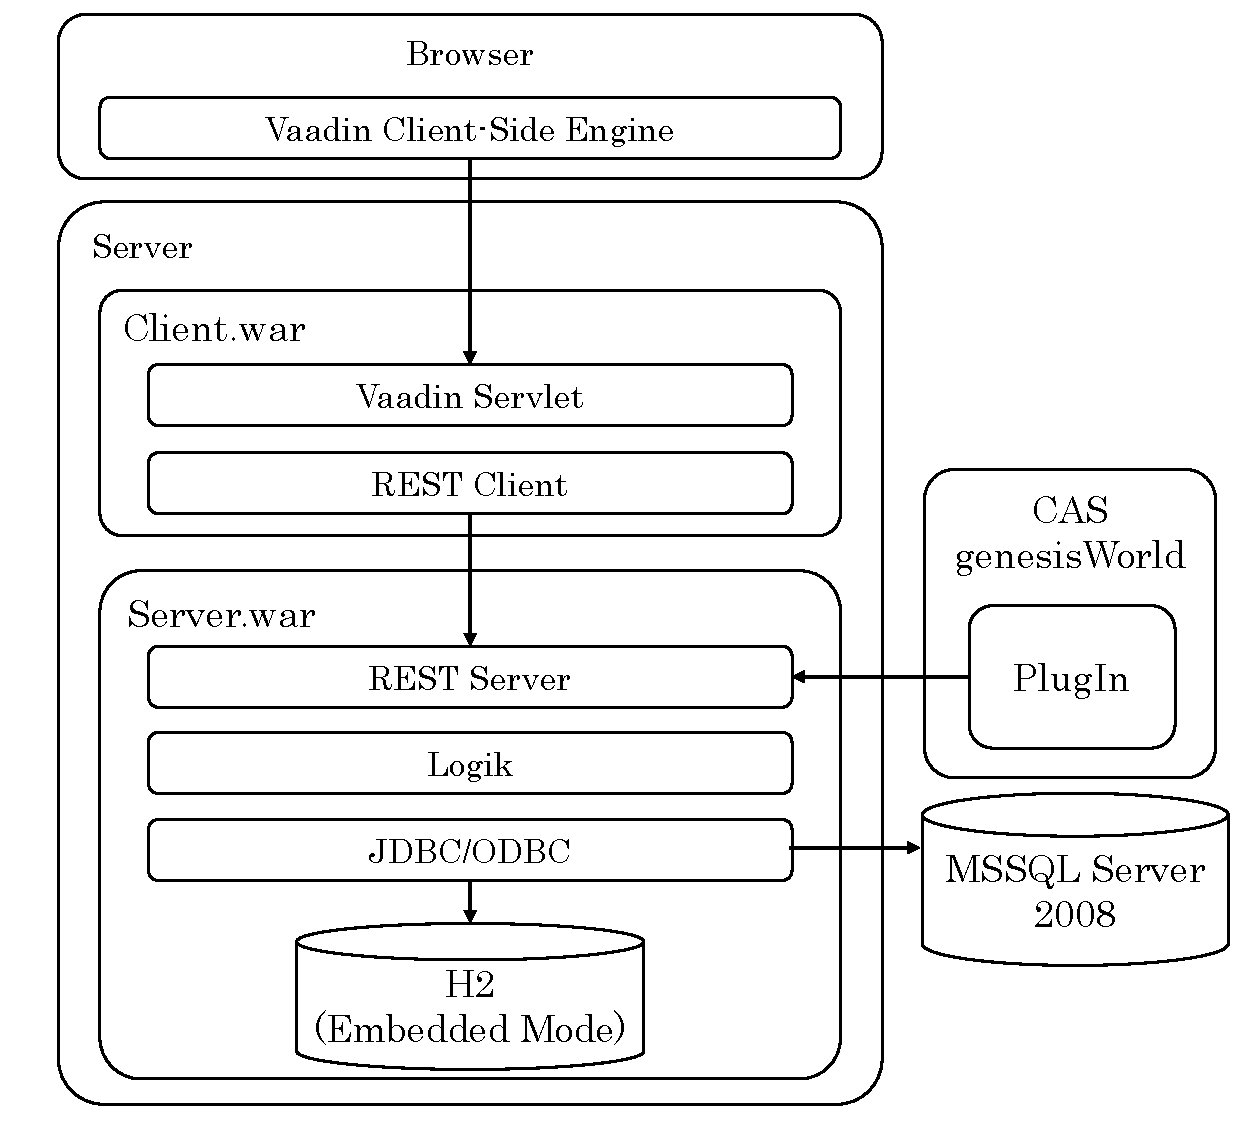
\includegraphics[width=0.8\textwidth, width=0.8\textwidth]{pics/Konzept_architektur.pdf}
\caption{Komponenten des Systems und der Umwelt}
\label{konzept_architektur}
\end{figure} 

\paragraph{Vaadin Client-Side-Engine}

Die Vaadin Client-Side-Engine verwaltet das Rendering der Oberfläche im Web-Browser.  Dies geschieht durch den Einsatz verschiedener clientseitiger Widgets, die das Gegenstück zu den serverseitigen Vaadin-Komponenten bilden. Es leitet Benutzerinteraktionen an die Serverseite weiter und rendert anschließend die Änderungen für die Benutzeroberfläche. Die Kommunikation findet über asynchrone HTTP-oder HTTPS-Anfragen statt. Weiterhin wird die Komponente durch Vaadin automatisch erzeugt und wird daher als gegeben betrachtet.

\paragraph{Client-Webprojekt}

Die Oberfläche des Systems wird durch ein Vaadin-Projekt realisiert. Mit dessen Hilfe werden die Bedien- und Darstellungselemente der Anwendung definiert. Sie ist außerdem für die Interaktion mit dem Benutzer zuständig. Die Delegation von verschiedenen Clients beispielsweise wird von einem Vaadin-Servlet erledigt. Dazu zählt das Empfangen von Anfragen und deren Zuordnung zu einer Sitzung des jeweiligen Benutzers. Die Elemente der Oberfläche selbst werden in Java geschrieben. Mithilfe der Java-Klasssen wird zur Laufzeit eine Javascript basierte Homepage erzeugt. Die Übersetzung von Java auf Javascript übernimmt Vaadin.

Das Server-Webprojekt ist eine weitere Komponente mit der interagiert werden soll. Die Kommunikation zwischen den beiden Komponenten soll über das REST-Protokoll stattfinden. Dazu implementiert das Client-Webprojekt einen REST-Client. Die Verwendung des REST-Protokolls zwischen dem Client-Webprojekt und Server-Webprojekt stellt überdies einen weiteres Element der losen Kopplung dar.

Ein Prozess in dem die einzelnen Bestandteile Verwendung finden, könnte wie folgt aussehen: Die Interaktionen der Benutzer mit der Oberfläche würden Events erzeugen, die zunächst auf der Clientseite durch Widgets verarbeitet werden. Nachfolgend würden die Events durch den HTTP-Server an das Vaadin-Servlet übergeben werden. Dieser leitet die Events an die entsprechenden Vaadin-Objekte weiter, bis sie zu den in der Anwendung definierten Event-Listenern gelangen. In den Listenern werden anschließend die REST-Clients aufgerufen. Mit Hilfe der REST-Clients werden die Eingaben der Nutzer an das Server-Webprojekt übermittelt. 

\paragraph{Server-Webprojekt}

Die eigentliche Lösung der Problemstellung soll im Server-Webprojekt des Softwaresystems implementiert werden. Es soll vollständig auf Java basieren. In ihr werden sich Klassen und Methoden befinden die eine Ermittlung der Informationen aus der H2-Datenbank ermöglichen. Zur Bestimmung der SQL-Parameter soll ein REST-Server implementiert werden, der die Beinutzeingaben entgegennimmt. Der REST-Server ist außerdem für die Kommunikation mit dem Plugin zuständig.

Weiterhin soll das Projekt sämtliche ETL-Prozessschritte implementieren. Die genauen Prozessschritte werden in Abschnitt \ref{ch:konzeption:etl} behandelt. 

%Die Logikkomponente in der Architektur stellt eine Zusammenfassung aller Funktionen des Anwendungskerns dar. Sie kümmert sich um die Generierung der Abfragen, welche an die Datenbank gestellt werden. Dabei erfolgt eine dynamische Generierung der Abfragen, um nicht durch unnötige Bedingungen die Verarbeitungsgeschwindigkeit zu verringern. Abfragen werden mithilfe der Java Database Connectivity (JDBC) an die Datenbank gestellt. Neben den Funktionen zur Abfragegenerierung enthält die Logikkomponente Prozesse zum Extrahieren und Transformieren von Daten aus der MSSQL-Datenbank. Der ETL-Prozess wird nur einmalig ausgeführt, allerdings stellt er einen wichtigen  Schritt für die Umsetzung dar. 


%In der Server.war werden REST-Requests entgegen genommen. Anhand der mitübertragenen Filteroptionen werden die Bedingungen für die Datenbankabfrage zusammengestellt. Anschließend wird eine Verbindung zur H2-Datenbank aufgebaut. Das Ergebnis der Abfrage wird in das JSON-Format überführt und zurück an die Client.war geschickt. Dort angekommen werden die Daten an die Vaadin-Komponenten übergeben, was einen Neuaufbau der entsprechenden Seitenbereiche bewirkt.      

\paragraph{H2-Datenbank}

Die H2-Datenbank ist als ein Bestandteil des Server-Webprojektes geplant. Dies ist durch den Betrieb im Embbeded-Modus möglich. Dadurch kann direkt aus dem Java-Code heraus mit der Datenbank gearbeitet werden. Um möglichst kurze Antwortzeiten zu Erreichen soll die In-Memory-Variante der Tabellen verwendet werden.

\paragraph{CAS genesisWorld Plugin} Systeme die auf dem Datenbestand anderer Systeme aufbauen können zwei verschiedene  Ansätze zur Sicherstellung ihrer Aktualität verfolgen. Unser nebenläufiges System bezeichnen wir als A und den CAS genesisWorld Anwendungsserver als B. Einer der Ansätze ist die Intervall basierte Nachfrage über Veränderungen von A. Hierbei fragt A bei B zu festgelegten Zeitpunkten nach, ob Daten verändert wurden. Die Definition eines optimalen Intervalls stellt eine der größten Schwierigkeiten dar. Ist der Intervall zu groß, sinkt die Aktualität des Datenbestandes. Ist er zu klein, entsteht eine starke Belastung für B. Der andere Ansatz ist A über Veränderungen an den Datensätzen von B zu informieren. Dadurch werden keine unnötigen Abläufe angestoßen, da nur im Falle einer Manipulation eines Datensatzes Prozesse in Bewegung gesetzt werden. Zwar wird die Aktualität der Daten gewährleistet, jedoch büßt A an Entscheidungsfreiheit ein. A kann nicht mehr selbst entscheiden wann aktualisiert wird. Der zweite Ansatz ist zwar effizienter, allerdings nicht immer umsetzbar. Das kann technische oder unternehmenspolitische Gründe haben, die notwendige Veränderung am Legacy-Systems ausschließen.  

In CAS genesisWorld gibt es die Möglichkeit den zweiten Ansatz umzusetzen. Die Idee dabei ist den CAS genesisWorld Anwendungsserver um ein Plugin zu erweitern, welches über Veränderungen in den Datensätzen benachrichtigt wird. Das Plugin soll über einen REST-Client die \textit{GGUID} des betroffenen Datensatzes an den Server-Webprojekt senden. Dort soll eine Kontrolle stattfinden, die den Datensatz auf Relevanz überprüft. Wird eine Relevanz festgestellt besorgt sich das Server-Webprojekt, anhand der zuvor übermittelten GGUID, alle benötigten Daten.

%% ===========================
\section{Datenbankdesign}
%% ===========================

Das Datenbankdesign stellt einen wichtigen Abschnitt in der Konzeption dar. An dieser Stelle werden Festlegungen im Bereich des Datenmodells getroffen. Sie entscheiden, ob Anforderungen und Erwartungen erfüllt werden können. Weiterhin werden die Charakteristika der Daten untersucht und das Datenmodell entsprechend nach ihnen gestaltet.

%% ===========================
\subsection{Konzeptionelles Design}
%% ===========================

Zunächst wird auf das geplante Schema der H2-Datenbank eingegangen. Indessen werden die Überlegungen und Entscheidungen die zur Entstehung des Schemas geführt haben erläutert. 

Die Normalisierung dient der Organisation von Feldern und Tabellen einer relationalen Datenbank, um Redundanz und Abhängigkeit zu minimieren. Die Kehrseite hingegen, ist eine Steigerung des Aufwands, um die benötigten Daten wiederzugewinnen. Normalisierung bietet dem Designer die Möglichkeit einen Austausch zwischen Performance und Stabilität des Datenbankmodells vorzunehmen \cite{geisler2011datenbanken}. Im neuen System stellt ersteres absolute Priorität dar. Daher soll die Normalisierung so gering wie möglich gehalten werden. 

Die erste Überlegung hinsichtlich des Schemas führt zu der Frage, welche Daten zur Umsetzung des Systems beibehalten werden. Der Datenbankdesigner steht bei analytischen System immer wieder vor der Entscheidung, wie viele Informationen aus dem alten System in das neue System übernommen werden sollten. Um höchstmögliche Verarbeitungsgeschwindigkeiten zu erreichen, werden lediglich die für das Szenario benötigten Daten extrahiert. Abbildung \ref{konzept_SchemaNeu} zeigt das für die Datenbank neu entworfene Schema. 

\begin{figure}[htbp]
\centering
  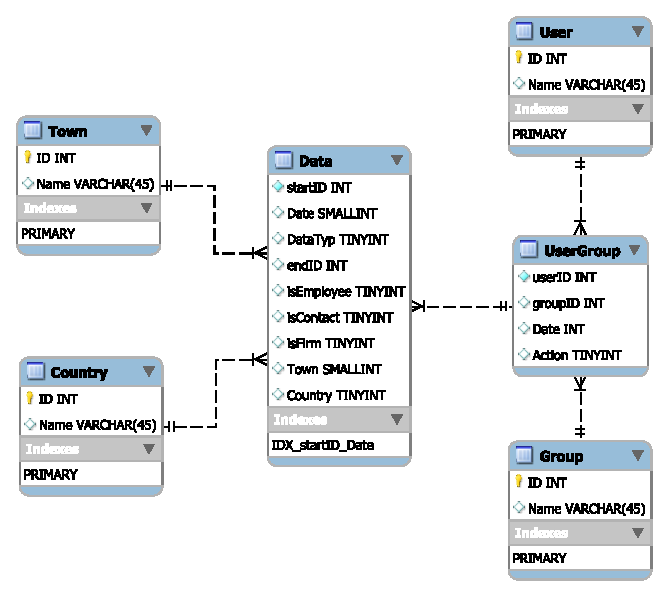
\includegraphics[width=0.8\textwidth, width=0.8\textwidth]{pics/NewSchema.pdf}
\caption{Neues Datenbankschema}
\label{konzept_SchemaNeu}
\end{figure} 

Die Idee hinter dem Schema ist die Verwendung einer einzelnen Tabelle zur Aufbewahrung der Informationen über die CRM-Objekte, die unter Personen geteilt werden. Diese Tabelle ermöglicht es ausgehend von einer Person alle CRM-Objekte die zu anderen Personen führen zu ermitteln. Die ersten vier Spalten werden benötigt, um die Anzahl der CRM-Objekte zwischen Personen festzustellen. Die erste Spalte \textit{startID} beinhaltet die Person von der die Bewertung ausgeht. Eine Zuordnung der Tupel zu einem Datum erfolgt über die Spalte \textit{Date}. Um CRM-Objekte zu unterscheiden, werden Zahlen von eins bis fünf in der Spalte \textit{DataTyp} für die jeweiligen Objekte verwendet. Die letzte Spalte \textit{endID} beinhaltet die ID der Personen mit der das CRM-Objekt geteilt wird. Alle anderen Spalten, wie \textit{Town} oder \textit{Country}, dienen dem Ausschluss von Personen aus der Abfrage.

Um mit den geringeren Speicherkapazitäten des Hauptspeichers zurechtzukommen, wird auf das Problem der Datenredundanz eingegangen. Durch Normalisierung lässt sich Datenredundanz zwar nicht verringern, allerdings kann man sie in kontrollierbare Bahnen lenken. Im neuen Schema werden solche Maßnahmen auf die Spalte \textit{Town} und \textit{Country} angewendet. 

Die Spalte \textit{Country} beispielsweise wird voraussichtlich Millionen von Werten beinhalten, jedoch gibt es im Vergleich nur wenige Länder auf der Welt. Die Ländernamen werden sich daher sehr oft wiederholen. Der Datentyp Varchar benötigt pro Zeichen 2 Byte an Speicherplatz. Aufgrund der stetigen Wiederholung von gleichen Wörtern ist die Verwendung von Varchar an dieser Stelle ungeeignet. Angesichts dessen werden die Ländernamen in einer eigenen Tabelle aufbewahrt. In dieser wird jedes Land nur einmal vermerkt und bekommt einen Primärschlüssel in Form einer Zahl. In der Tabelle \textit{Data} wird dann nur noch der jeweilige Fremdschlüssel verwendet. Das würde zum Beispiel bei dem Wort "Deutschland" eine Reduktion von 22 Byte auf 1 Byte bewirken. Die Reduzierung auf 1 Byte entsteht durch die Verwendung des Datentyps tinyint. Das alles gilt ebenfalls für die Spalte \textit{Town}. Bei ihr wird allerdings der Datentyp smallint verwendet, da dessen Zahlenbereich von -32768 bis 32767 reicht. Damit lassen sich alle Städte aus der MSSQL-Datenbank abdecken. 

Die Spalten \textit{isEmployee}, \textit{isContact} und \textit{isFirm} können nur zwei verschiedene Zustände darstellen. Trifft zu oder trifft nicht zu. Der Datentyp \texttt{bool} reicht daher zur Abbildung der zweiwertigen Zustände aus. Ein Feld vom Datentyp datetime benötigt 8 byte an Speicher. Um hier ebenfalls Einsparungen vorzunehmen, wurde beschlossen das Datum als smallint zu deklarieren. Dies ist möglich, weil nur der Tag des Datums von Interesse ist. Dazu wird ein frei gewählter Nullpunkt festgelegt. In unserem Fall wurde der 01.01.1990 als Nullpunkt gewählt, da keine älteren Daten existieren, die eine Relevanz besitzen. Der Wert eines Datum wird durch die Anzahl der Tage seit dem Nullpunkt ermittelt. Ein Beispiel wäre der 05.01.1990 der in der Spalte als 4 vermerkt werden würde. Die Hochrechnung der Tabelle \ref{tb_speicherplatzverbrauch} zeigt, dass durch die Normalisierung der Speicherplatzverbrauch um bis zu $ \frac{1}{6} $ gesenkt werden kann.

\begin{table}[htbp]
\centering
\begin{tabulary} {\linewidth} {l  r  C  l  C  r}
& & & & & \\
\multicolumn{6}{l}{Speicherplatzverbrauch ohne Normalisierung}\\
& & & & & \\
Zeitpunkt(timestamp) & 8 byte & x & 18.000.000 & = & \textasciitilde 137 MB \\  
Stadt(varchar) & 16 byte & x & 18.000.000 & = & \textasciitilde 343 MB \\  
Land(varchar) & 20 byte & x & 18.000.000 & = & \textasciitilde 274 MB \\  
\midrule
& & & & Summe & \textasciitilde 754 MB\\
& & & & & \\
\multicolumn{6}{l}{Speicherplatzverbrauch mit Normalisierung}\\
& & & & & \\
Zeitpunkt(smallint) & 2 byte & x & 18.000.000 & = & \textasciitilde 34 MB \\  
Stadt(integer) & 4 byte & x & 18.000.000 & = & \textasciitilde 72 MB \\  
Stadt(varchar) & 16 byte & x & 21.000 & = & \textasciitilde 0,32 MB \\  
Land(tinyint) & 1 byte & x & 18.000.000 & = & \textasciitilde 17 MB \\  
Land(varchar) & 20 byte & x & 218 & = & \textasciitilde 0,004 MB \\
\midrule  
& & & & Summe & \textasciitilde 123 MB\\
& & & & & \\
\end{tabulary}
\caption{Vergleich des Speicherplatzverbrauchs}
\label{tb_speicherplatzverbrauch}
\end{table}

Durch die zusätzlichen Tabellen kann zwar Speicherplatz gespart werden doch nun muss überlegt werden wie die Informationen wiederbeschafft werden sollen. Wird eine Benutzerabfrage gestellt die eine Filterung anhand einer Stadt voraussieht, wird zuerst die \textit{ID} der Stadt benötigt. Dabei können zwei verschiedene Ansätze verfolgt werden. Der erste Ansatz wäre ein Verbund zwischen \textit{Town} und \textit{Data}, um direkt mit dem Namen der Stadt zu arbeiten. Diese Variante dürfte aufgrund des Kreuzproduktes von Millionen von Zeilen nicht sehr performant sein. Eine andere Möglichkeit wäre eine separate Abfrage an die Datenbank zu stellen, in der die \textit{ID} zum Namen ermittelt wird. Mithilfe der \textit{ID} kann dann ohne einen Verbund die Ergebnismenge ermittelt werden. Dieser Ansatz dürfte zu geringeren Antwortzeiten führen, da keine Verzögerungen durch Netzwerkzugriffe entstehen. Dieses Vorgehen kann für die Stadt, das Land und die Gruppenzugehörigkeit angewendet werden.

Die Tabelle \textit{GroupDate} unterscheidet sich von den anderen Tabellen wie \textit{Town} oder \textit{Country}, da in dieser noch weitere Details vermerkt sind. Diese ermöglichen es die Zusammenstellung von Gruppen über die Zeit nachzuvollziehen. In der Spalte \textit{Action} wird festgelegt, ob die Tupel einen Eintritt oder einen Austritt einer Person darstellt. Die Spalte \textit{Date} beinhaltet das Datum des Ereignisses. Mithilfe beider Attribute lassen sich Gruppenzusammensetzung auf bestimmte Zeitpunkte bezogen rekonstruieren.

%% ===========================
\subsection{Zugriffsstrukturen}
%% ===========================

Zum Beschleunigen der Zugriffe auf die Datensätze der H2-Datenbank wird auf die beabsichtigten Zugriffsverfahren eingegangen. 

Indizes werden zur Beschleunigung von Suchen nach bestimmten Spaltenwerten eingesetzt. Ohne Indizes müsste die H2-Datenbank beim ersten Datensatz beginnen und dann die gesamte Tabelle durchgehen, um eine Abfrage zu beantworten. Je größer die Tabelle ist, desto höher ist der Aufwand dafür. Der Einsatz von Indizes ist in Anbetracht der Zielsetzung von kurzen Antwortzeiten ein interessantes Hilfsmittel. Jeder Index bedeutet allerdings einen Zuwachs im Speicherplatzverbrauch. Zur Indexierung der Tabellen \textit{Town},\textit{UserGroup}, \textit{Country}, \textit{User} und \textit{Group} eignen sich Hash-Indizes. Sie bieten einen extrem schnellen Zugriff auf die Daten. Diese Schnelligkeit ergibt sich aus der Verwendung von Berechnungsvorschriften, zur Ermittlung der Position des gesuchten Wertes. Indizierungen sollen im vorliegenden Schema über die Spalten mit der Bezeichnung \textit{Name} vorgenommen werden, da der Client mit dem Namen anstatt mit der ID arbeitet. Mithilfe des Namens wird anschließend die zugehörige ID ermittelt. Die Nutzung von Hash-Indizes bringt allerdings Limitierungen mit sich. Eine der wichtigsten ist, dass sie nur für Vergleiche ("=") verwendbar sind. Somit werden keine Wertebereichabfragen ("<" oder ">") unterstützt. Es gibt allerdings noch andere Nachteile \cite{SWB-352401869}, auf die aber in dieser Arbeit nicht näher eingegangen wird. 

Für die Tabelle \textit{Data} eignet sich der B\textsuperscript{+}-Baum-Index. Er ermöglicht eine effizientere Ausführung der Grundoperationen wie Suchen, Einfügen und Löschen. Die Spalte \textit{startID} und \textit{Date} eignen sich am besten für die Indexierung. Dabei handelt es sich um einen Mehr-Attribut-Indexe, da wir zwei Attribute verwenden. Der Vorteil eines Mehr-Attribut-Indexes ist, dass bei einer Punkt-Abfrage über alle Zugriffsattributwerte nur ein Indexzugriff erfolgen muss.
Beide Spalten sind sortiert und bieten sich somit für die Verwendung von einem geclusterten Index an. Ein Geclusterter Index ist in der gleichen Form sortiert wie die interne Relation. Dadurch unterstützt bietet er eine sehr gute Unterstützung für Bereichsabfragen. Dieser Vorteil kann in der Spalte Date ausgenutzt werden, da in den Abfragen immer ein bestimmter Zeitraum betrachtet wird.


%% ===========================
\section{ETL-Prozess}
\label{ch:konzeption:etl}
%% ===========================

Daten der operativen Systeme unterstützen die wertschöpfenden Geschäftsprozesse innerhalb eines Unternehmens. Sie sind demnach auf die Steuerung und Überwachung des Tagesgeschäftes ausgerichtet und daher transaktionsbezogen. Somit sind die Daten in ihren Begrifflichkeiten häufig nicht vergleichbar und ihrer Bewertung sowie Konsolidierung unterschiedlich. Um die Daten dennoch für analytische Zwecke einzusetzen, ist eine Überführung in eine geeignete Struktur von Vorteil. Eine solche Überführung wird in der Literatur als Extract-Transform-Load (ETL)-Prozess bezeichnet \cite{ElSappagh201191}. 

Abbildung \ref{konzept:etl} zeigt das erarbeitete Konzept zur Umsetzung eines solchen ETL-Prozesses. In den nächsten drei Abschnitten wird jeder ETL-Schritt näher erläutert.

\begin{figure}[htbp]
\centering
  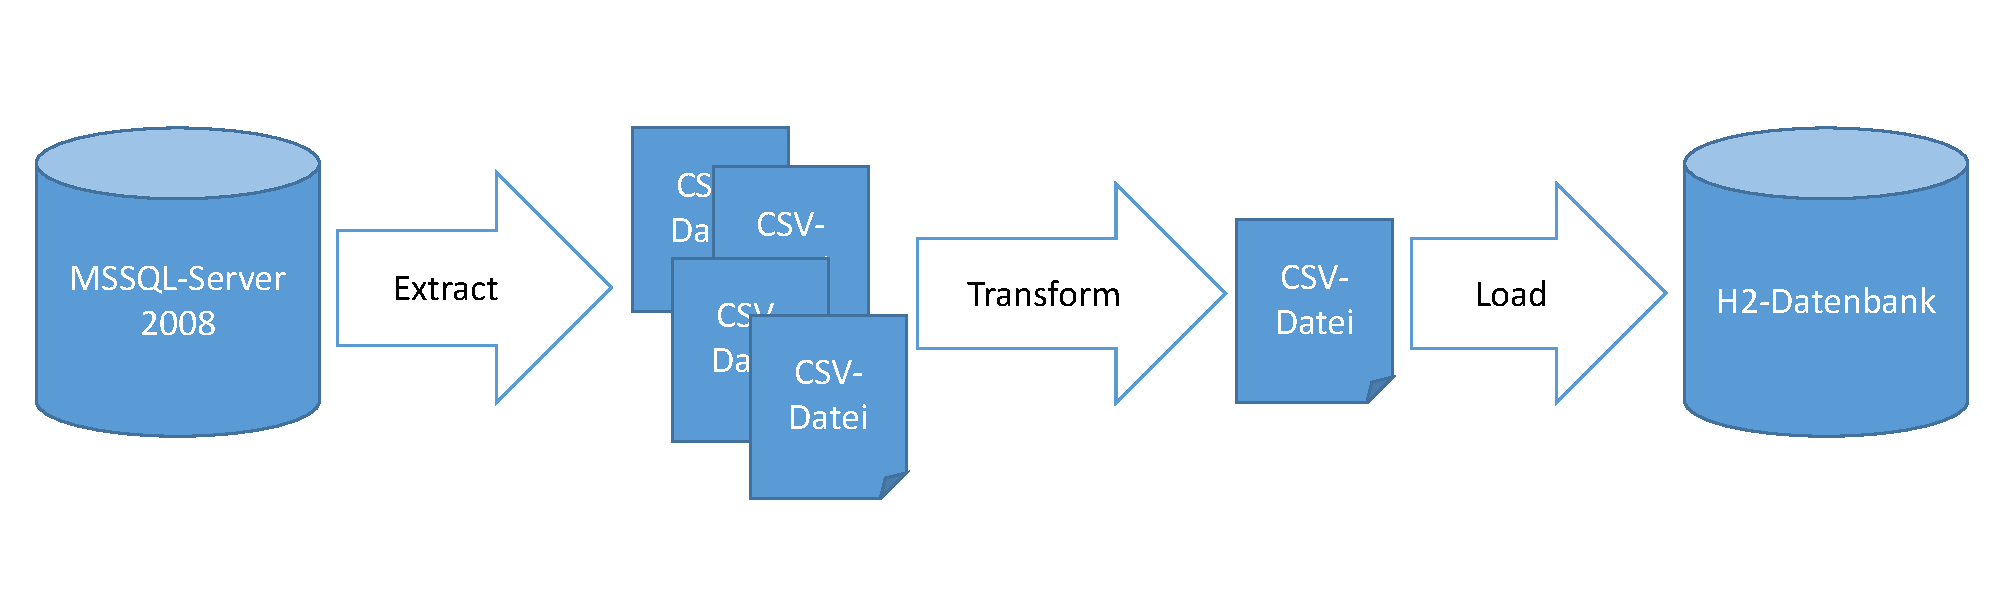
\includegraphics[width=1.0\textwidth, width=1.0\textwidth]{pics/ETL.pdf}
\caption{ETL-Prozess}
\label{konzept:etl}
\end{figure} 


%% ===========================
\subsection{Extract}
\label{ch:konzeption:etl:extract}
%% ===========================

Zunächst dient die Extraktion primär der Beschaffung von Daten aus der MSSQL-Datenbank. Überdies können durch den Prozess Daten bereits reduziert,  zusammengeführt und ersetzt werden. Für eine zutreffende Formulierung der Abfragen müssen Besonderheiten in die Ermittlung der Daten beachtet werden. Eine vollständige und korrekte Datenmenge stellt die Grundlage jeder guten Analyse dar.

In der Extraktion sollen SQL-Abfragen formuliert werden mit denen die Daten aus der MSSQL-Datenbank in die H2-Datenbank überführt werden können. Dabei gilt es die Abfragen so zu formulieren, dass das Ergebnis den Attributen aus der Tabelle des neuen Schemas entspricht.

Weiterhin sind Besonderheiten in der Extraktion zu beachten. Es existieren Datensätze in der MSSQL-Datenbank die sich über längere Zeiträume erstrecken. Beispielsweise erstrecken sich Termine wie Tagungen über mehrere Tage. In der MSSQL-Datenbank werden diese Termine in einer Tupel aufbewahrt. Bei unserer Analyse hingegen stellt jede Tupel eine Verbindung zu einem bestimmten Tag dar. Somit muss ein Datensatz der sich über mehrere Tage erstreckt, in der H2-Datenbank durch mehrere Tupeln repräsentiert werden. Aufgrund dessen wird im Ergebnis der SQL-Abfrage die Zeitspanne eines CRM-Objektes in Tagen vermerkt. In späteren Transformationen kann mithilfe dieser Angaben die entsprechende Anzahl an Tupeln erzeugt werden.

Eine weitere Besonderheit ergibt sich durch eine Funktionalität von CAS genesisWorld, welche es ermöglicht Termine zu schieben. Diese Funktion wird von manchen Nutzern missbraucht. Anstatt für einen ähnlichen Termin einen neuen Eintrag anzulegen, wird ein alter Termin aus Bequemlichkeit geschoben. Das hat zur Folge, dass Termine die tatsächlich stattgefunden haben, in der Datenbank nicht mehr existieren. Um trotzdem diese Termine zu berücksichtigen wurde folgendes Konzept erarbeitet. 

Dem \textit{Changelogbook} lassen sich Veränderungen von Feldern entnehmen. Um Schiebungen zu erkennen werden die Änderungen in den Spalten \textit{start\_dt} und \textit{end\_dt} benötigt. Zur Feststellung ob ein Termin stattgefunden hat und anschließend geschoben wurde, müssen drei Bedienungen erfüllt sein. Die erste ist der Zeitpunkt der Schiebung, der nach dem Termin liegen muss. Wird ein Termin aus anderen Gründen geschoben findet dies in der Regel vor dem Start des Termines statt, damit die Personen nicht unnötig zum Termin erscheinen. Die zweite Bedingung ist, dass der neue Termin in der Zukunft liegen muss. Neben den beiden zuvor genannten Bedingungen muss die Operation auf den Datensätzen ein Update gewesen sein. Nur dann ist der Datensatz von Relevanz für die Ermittlung der geschobenen Termine. 

Die Ergebnisse sämtlicher Extraktionen werden in CSV-Dateien abgespeichert. Damit werden unteranderem eventuelle Fehlersuchen vereinfacht. Weiterhin wird die Belastung des Hauptspeichers verringert, da nicht alle Ergebnisse bis zum Ende der Extraktion in der Java-Laufzeitumgebung aufbewahrt werden müssen.

%% ===========================
\subsection{Transform}
%% ===========================

Zu Beginn der Transformation werden Filterungen durchgeführt. Unter der Filterung von operativen Daten versteht man eine Bereinigung syntaktischer oder inhaltlicher Defekte, der zu übernehmenden Daten. Die MSSQL-Datenbank besteht zu 37\% aus Nullwerten und zu 4\% aus leeren Feldern. Daten die beispielsweise Nullwerte enthalten und für die Ermittlung des Datums benötigt werden, sind für die Analyse nicht zu gebrauchen. Sie können daher im Laufe des Prozesses aus den Daten entfernt werden. Bei den anderen Filteroperationen können Nullwerte vernachlässigt werden, da sie zweckmäßig abdingbar sind.

Der nächste Schritt ist die Harmonisierung der Daten. Unter anderem besitzen die Telefonnummern kein einheitliches Format. Sie wurde manuell von Sachbearbeitern eingetragen. Zur Lösung des Problems werden aller Nummern in ein einheitliches Format gebracht, welches einen automatischen Vergleich ermöglicht. Die CRM-Objekte müssen ebenfalls in eine einheitliche Struktur gebracht werden. Sie besitzen alle die benötigten Informationen, allerdings werden diese unter Unterschiedlichen Bezeichnungen und eventuell in einem anderen Format aufbewahrt.

Die in der Extraktion genannten Besonderheiten werden durch unterschiedliche Datenbankabfragen ermittelt. Dies führt zu vielen separaten Dateien. Zur Nutzung der Daten sind diese zum Abschluss der Transformation zu sortieren und zusammenzuführen. Das Ergebnis wird anschließend in einer CSV-Datei gespeichert, welche die Basis zum Einspielen der Daten in die H2-Datenbank bildet. 

%% ===========================
\subsection{Load}
%% ===========================

Beim Laden der Datensätze in die H2-Datenbank kommt ein sogenannter "bulk load" zum Einsatz. Dieser wird häufig zum Laden von großen Datenmengen aus einer Datei in eine Datenbank eingesetzt. Er ermöglicht ein wesentlich schnelleres einspielen von großen Datenmengen in die Datenbank, gegenüber der Verwendung von INSERT-Operatoren.

%% ===========================
\section{Entwurf der Oberfläche}
\label{ch:Konzeption:sec:Darstellungskonzepte}
%% ===========================

Bei der Konzeption einer Darstellung ist der Detaillierungsgrad von Informationen ein wichtiger Leitfaden. In unserem Fall ist nicht die Eigenschaft eines CRM-Objekts von interessiere, sondern ihr Typ und ihre Häufigkeit. Da keine detaillierten und privaten Informationen zu den CRM-Objekten aufbewahrt werden, kann jeder Benutzer frei wählen von welcher Person die Bewertung ausgehen  soll. Für die Oberfläche bedeutet dies einen Einstiegspunkt in Form eines Fensters in dem der Benutzername einer Person, von dem die Suche ausgehen soll, eingegeben wird. Zusätzlich soll eine Möglichkeit bestehen die IP-Adresse und Portnummer des Servers anzugeben, um den Client auf anderen Rechnern betreiben zu können.

Nach der Anmeldung findet eine Weiterleitung auf die eigentliche Seite statt. Dessen Aufbau ist in Abbildung \ref{konzept_darstellung} zu sehen. Im oberen Bereich auf der Seite sind alle Regler, CheckBoxen und Eingabefelder zur Filterung der Ergebnismenge zu finden. Direkt darunter befindet sich ein Diagramm, welches das Ergebnis der Abfrage visualisieren soll.

\begin{figure}[htbp]
\centering
  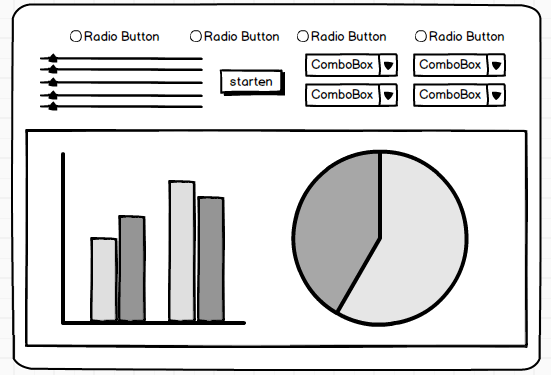
\includegraphics[width=0.8\textwidth, width=0.8\textwidth]{pics/mockup.png}
\caption{Entwurf der Oberfläche}
\label{konzept_darstellung}
\end{figure} 

In der Wahl eines Diagrammtypen ergeben sich allerdings Einschränkungen durch das verwendete Framework. Im Grunde lässt sich jede Darstellung umsetzen, jedoch ist das Aufwand-Nutzen-Verhältnis zu berücksichtigen. In einer Vorauswahl wurden einige  Typen ausgewählt, die in Abbildung \ref{konzept_darstellung2} dargestellt sind. 

Netzdiagramme (a) geben Eigenschaften verschiedener Systeme wieder. Sie eignen sich daher gut zur Darstellung von Ausprägungen. Für die vorliegenden Daten ist diese Darstellung gänzlich ungeeignet, da mit Mengen gearbeitet wird. 

Mithilfe von Liniendiagrammen (b) lassen sich Trends und Zeitreihen darstellen. Die Verwendung verschiedener Linien ermöglicht zudem die Darstellung mehrerer Trends. Die Benutzung dieses Diagramms wäre nicht sinnvoll, da die Ergebnismenge sich nicht auf verschiedene Zeitpunkte bezieht, sondern die Summe der Werte aus einer Zeitreihe beinhaltet. 

\begin{figure}[htbp]
\subfigure[Netzdiagramm]{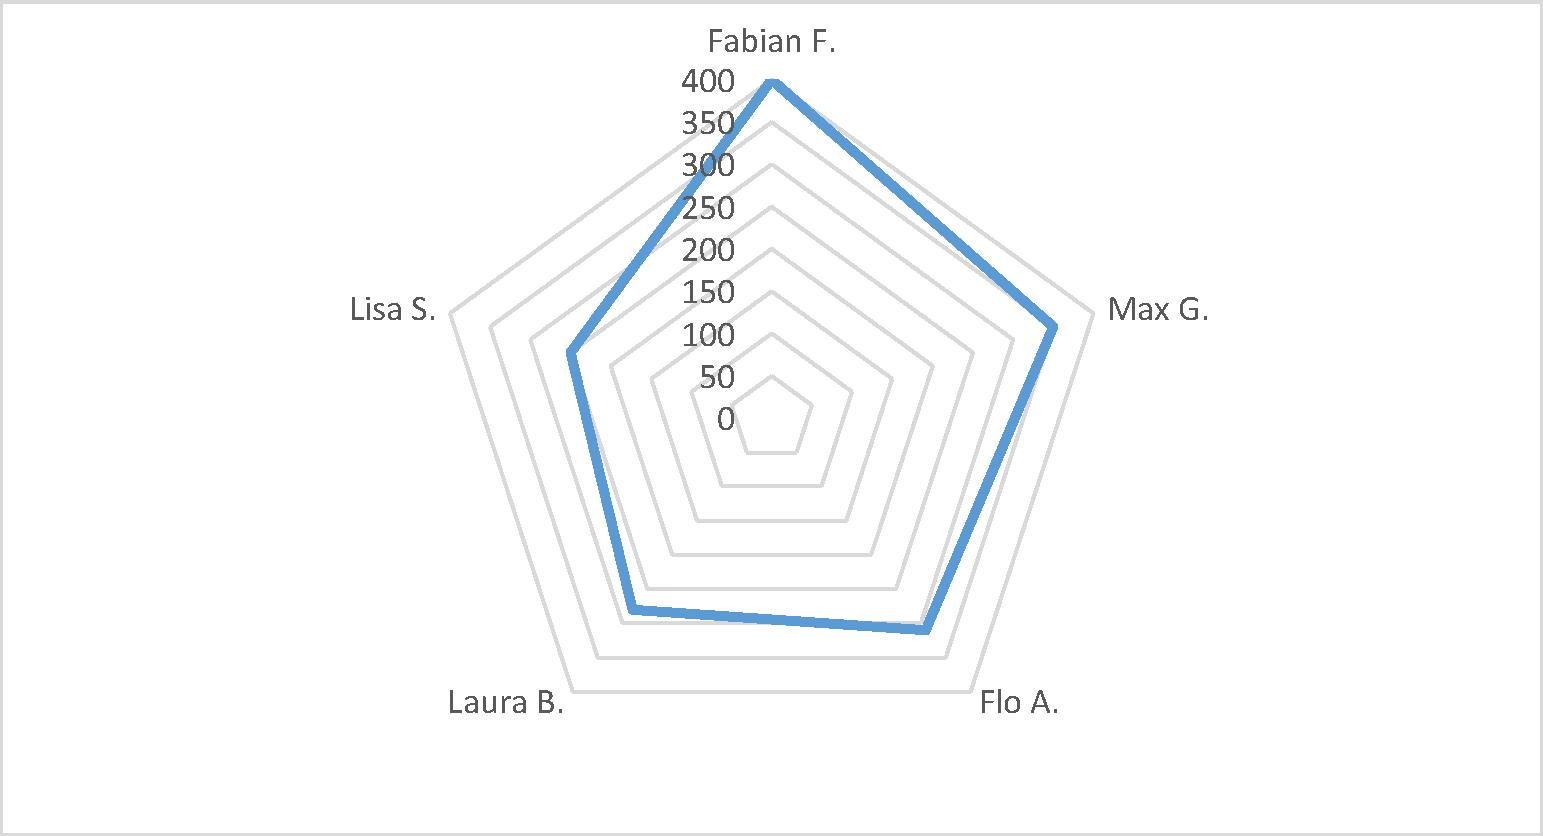
\includegraphics[width=0.3\textwidth]{pics/konzept_netzdiagramm.pdf}}\hfill
\subfigure[Liniendiagramm]{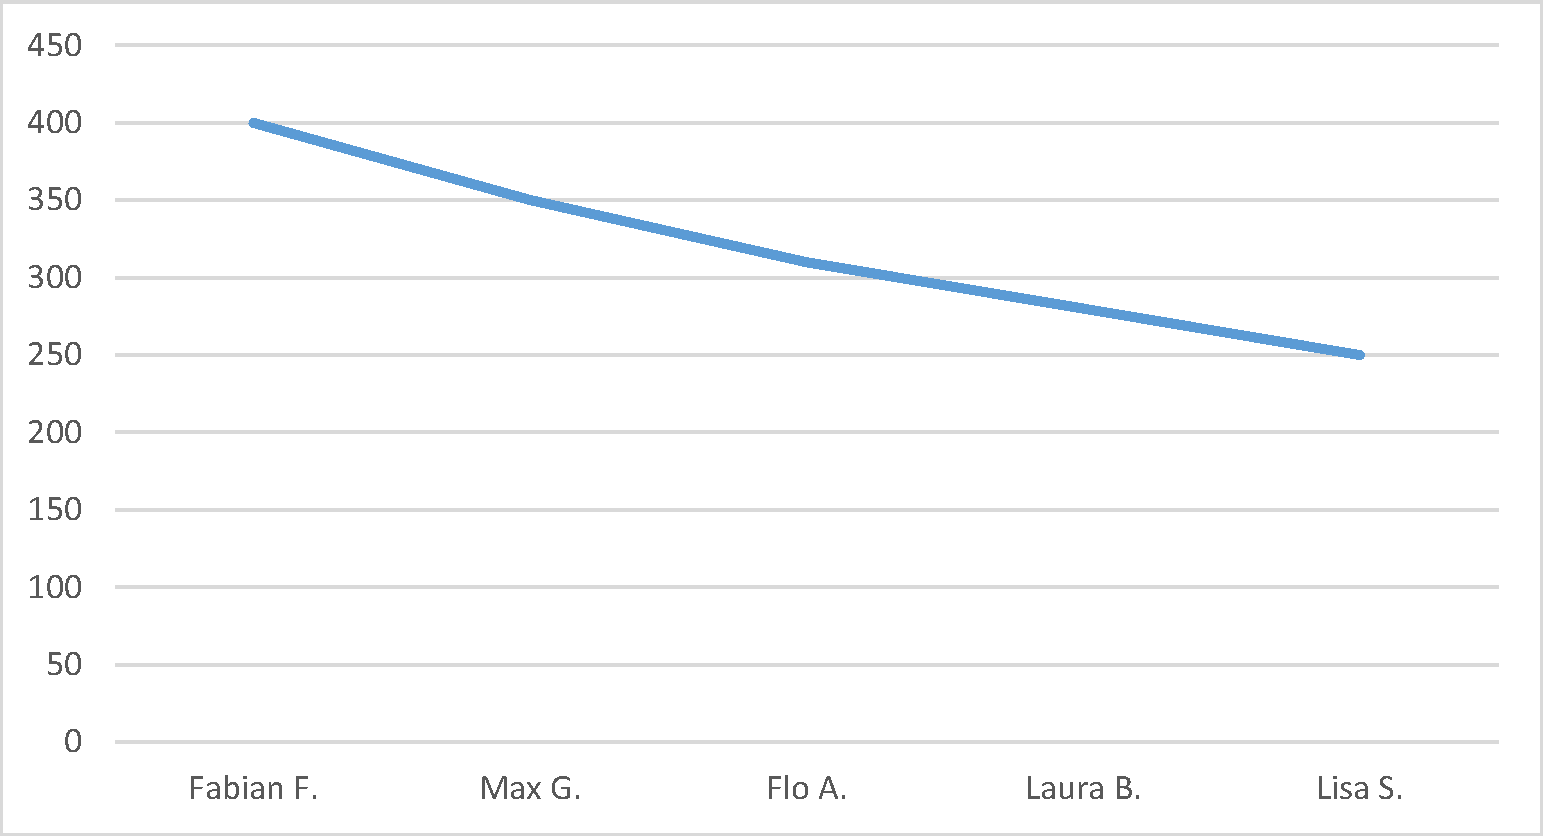
\includegraphics[width=0.3\textwidth]{pics/konzept_liniendiagramm.pdf}}\hfill
\subfigure[Tree Map]{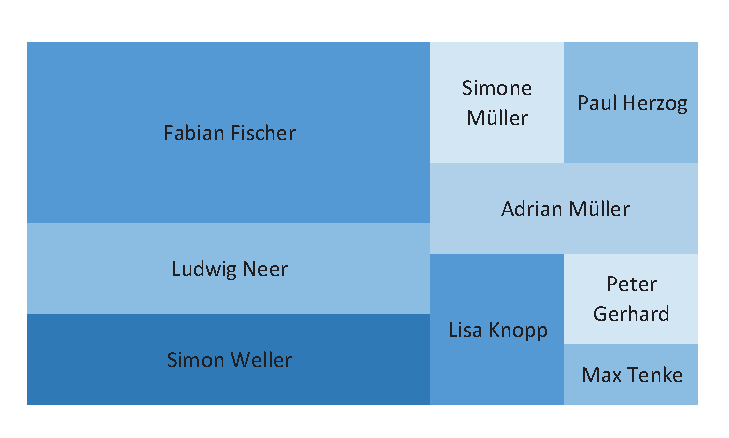
\includegraphics[width=0.3\textwidth]{pics/konzept_tree_map.pdf}}\hfill
\subfigure[Tortendiagramm]{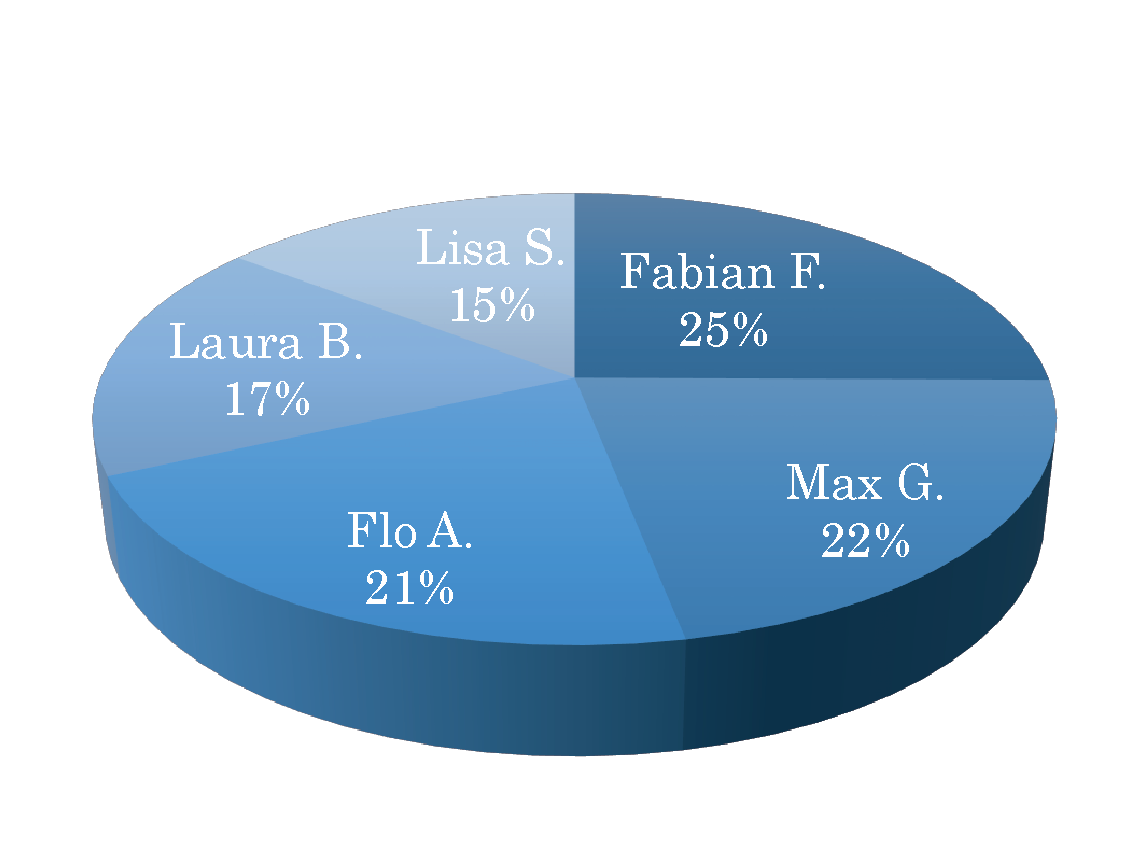
\includegraphics[width=0.3\textwidth]{pics/konzept_tortendiagramm.pdf}}
\subfigure[Balkendiagramm]{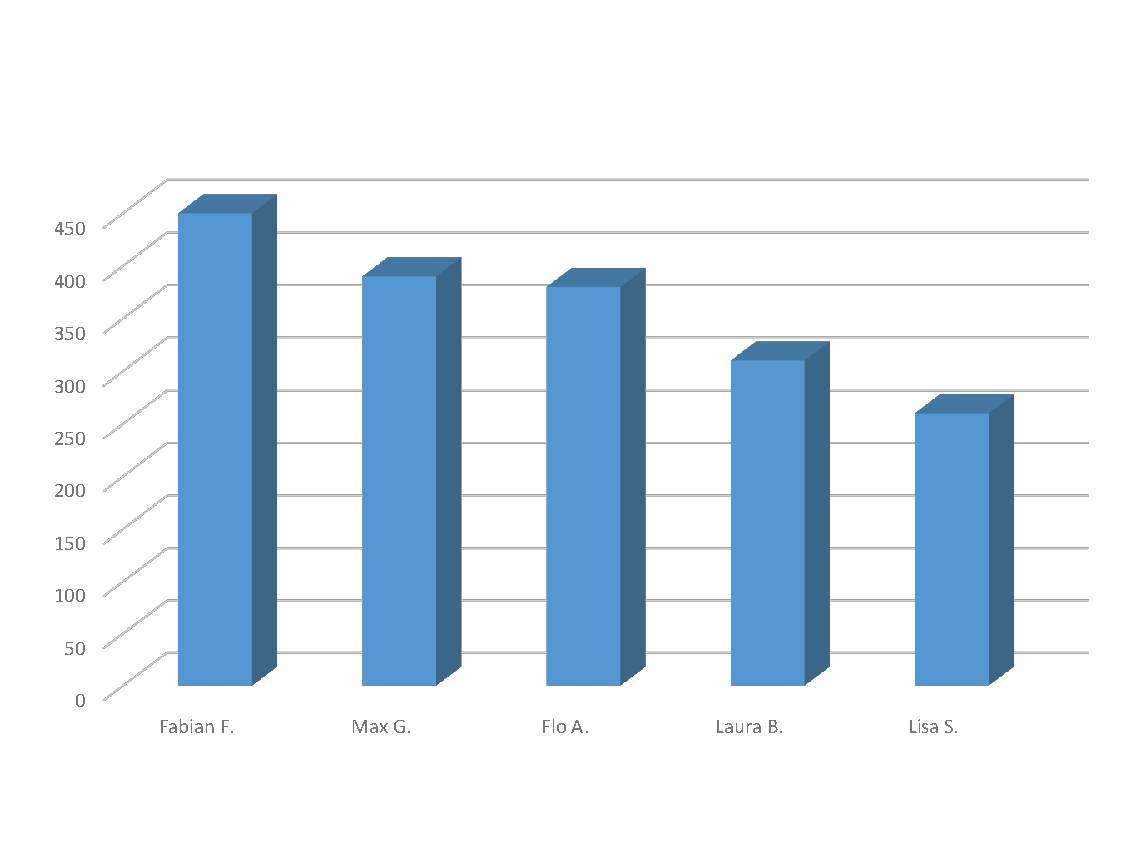
\includegraphics[width=0.3\textwidth]{pics/konzept_balkendiagramm.pdf}}
\caption{Entwürfe für die Oberfläche}
\label{konzept_darstellung2}
\end{figure}

Bei einer Tree Map (c) steht jede Fläche eines Rechtecks im proportionalen Zusammenhang zur Gesamtfläche. Die Beachtung von Größenverhältnissen stellt eine nützliche Eigenschaft für unsere Daten dar. In unserem Fall würde jedes Rechteck aus dem jeweiligen Anteilen der Verbindungsmerkmale bestehen oder mithilfe eines Drilldowns
\footnote{Als Drilldown wird im Allgemeinen die Navigation in hierarchischen Daten bezeichnet. Auf Oberflächen bezogen wird damit die Darstellung von Detailinformationen durch einem Klick auf Darstellungselemente ausgedrückt.}
 die Verbindungsmerkmale aufzeigen. Beispielweise könnte die Person Ludwig Neer wiederum in Rechtecke unterteilt werden, mit der jeweiligen Anzahl der verschiedenen Verbindungsmerkmale. Das würde allerdings aufgrund zu vieler Kacheln schnell zu einer schlechten Übersicht führen. Wird in einer Tree Map die Drilldown-Navigation gewählt, ist die Übersicht aller Informationen auf einen Blick nicht mehr gegeben. Aufgrund der Nachteile in der jeweiligen Variation wurde sich gegen den Einsatz einer Tree Map entschieden.

Kreisdiagramme (d) ermöglichen eine Betrachtung der Gesamtheit zu ihren Einzelstücken, da der Kreis ein geschlossenes System darstellt. Allerdings müssen sich alle Kreisstücke auf die gleiche Basis beziehen. Es eignet sich hervorragend zur Darstellung von Verhältnissen. Wird nun eine weitere Unterteilung der Teilwerte benötigt, geht die Übersicht verloren. Um das zu vermeiden wird die unterteilte Teilmenge häufig in separaten Ansichten dargestellt. Allerdings steigt dadurch der Aufwand für den Nutzer in der Bedienung des Systems. 

Das Balkendiagramm (e) ist für die Darstellung der Daten am geeignetsten. Reihenfolgen beispielsweise lasse sich durch die resultierenden Stufen sehr gut darstellen. Balken selbst lassen sich außerdem in einzelne Teile aufspalten, ohne die Übersichtlichkeit zu verringern. Gegenüber dem Kreisdiagramm kann es zwar keine Betrachtung des Gesamten liefern, allerdings ist das in diesem Anwendungsfall auch nicht nötig. 

%% ===========================
\section{Technologien}
%% ===========================

Als eine der am meist verbreitetsten Programmiersprachen, stellt Java die Grundlage aller verwendeten Technologien dar. Zur Darstellung der Inhalte für den Client wird Vaadin verwendet. Der Apache Tomcat nimmt die Rolle des Anwendungsservers ein. Die Kommunikation auf Basis von RESTful Web Services wird mithilfe von Jersey realisiert. Weiterhin wird opencsv für das Lesen und Schreiben von CSV-Dateien verwendet. JDBC wird zur Kommunikation zwischen dem Anwendungsserver und der Datenbank. Die H2-Datenbank stellt die Datenquelle des Systems dar. Im Folgenden werden alle Bestandteile, bis auf die bereits erläutert H2-Datenbank, näher beschrieben. 

\paragraph{Vaadin}

Vaadin ist ein Open-Source-Framework für den Aufbau von modernen Web-Anwendungen.
Es verwendet ein reines serverseitiges, eventbasiertes Modell und ermöglicht eine Anwendungsentwicklung ohne direkte Verwendung von HTML und JavaScript-Code. Das Framework ermöglicht es, die gesamte Anwendungslogik auf der Serverseite einer Anwendung auszuführen, während die Clientseite nur für das Senden der Benutzeraktionen an den Server und für die Reaktion auf die Antworten verantwortlich ist. Da es auf GWT basiert, kann sowohl der Client- als auch der Server-Code in reinem Java geschrieben werden.

Die aktuelle Version von Vaadin wurde im Februar 2013 veröffentlicht. Die folgenreichste Änderung von Vaadin6 war die Integration von GWT zu Vaadin, die eine bessere Unterstützung für die clientseitige Widget-Entwicklung bedeutet und sogar die Möglichkeit zum Erstellen von Offline-Anwendungen mit sich bringt.

Die im Unternehmen vorhandene Erfahrung und Open-Source stellen relevante Entscheidungsfaktoren in der Wahl von Vaadin. Allerdings war VaadinCharts, eine Erweiterung für Vaadin, für die Auswahl ausschlaggebend. Es basiert auf Highcharts, einem JavaScript-Packet. Highcharts zeichnet sich durch eine umfangreiche Sammlung an Funktionen zur Darstellung von Diagrammen aus. 

\paragraph{Jersey}

Jersey ist ein Open-Source-Framework zur Entwicklung von RESTful Web Services in Java, welches eine Unterstützung für JAX-RS-APIs bietet und die JAX-RS (JSR 311 und JSR 339)-Referenzimplementierung darstellt. JAX-RS-Annotationen werden verwendet um die Relevanz von Java-Klassen für REST zu definieren. Jersey enthält einen REST-Server und einen REST-Client. Auf der Serverseite verwendet Jersey ein Servlet zum Abtasten von vordefinierten Klassen, um REST-Ressourcen zu identifizieren. Über die web.xml Konfigurationsdatei werden die von der Jersey-Distribution bereitgestellten Servlets registriert. Diese Servlets analysieren die eingehenden HTTP-Nachrichten und wählen die richtige Klasse und Methode für die Anfragen aus. Diese Auswahl basiert auf Annotationen in diesen Klassen und Methoden. Weiterhin unterstützt JAX-RS die Erstellung von XML und JSON mithilfe der Java Architektur für XML Binding (JAXB).

\paragraph{Apache Tomcat7}

Tomcat ist ein Open-Source-Webserver, der von der Apache Group entwickelt wurde. Der Apache Tomcat implementiert die Java Servlets-, sowie die JavaServer Pages-Spezifikation von Sun Microsystems und stellt folglich eine Referenzimplementierung dar. Er stellt weiterhin eine rein auf Java-basierende HTTP-Webserverumgebung dar. Weiterhin kann der Tomcat über eine Oberfläche sowie durch Bearbeiten von XML-Dateien konfiguriert werden.

\paragraph{opencsv}

Da Java das Parsen von CSV-Dateien nativ nicht unterstützt, wird auf eine Drittanbieterbibliothek zurückgegriffen. Diese heißt opencsv und ist eine sehr einfache CSV-Parser-Bibliothek für Java. Die Bibliothek kann zum Erstellen, Lesen und Schreiben von CSV-Dateien verwendet werden. Die wichtigste Fähigkeit des opencsv-Parsers ist das Mapping von CSV-Daten auf Java-Bean-Objekte.

\paragraph{JDBC}

Die JDBC-API ermöglicht den programmgesteuerten Zugriff auf relationale Daten, direkt aus der Java Programmiersprache heraus. Durch die Verwendung der JDBC-API können Java-Anwendungen SQL-Anweisungen ausführen, Ergebnisse abrufen und die Veränderungen auf die Datenquelle zurückschreiben. Die JDBC-API kann auch mit mehreren Datenquellen in einer verteilten, heterogenen Umgebung interagieren. 
